\documentclass{beamer}
\usetheme{JLTree}

\usepackage{graphicx}
\usepackage[italian]{babel}
\usepackage[latin1]{inputenc}
\usepackage[T1]{fontenc}
\usepackage{amsfonts}
\usepackage{url}
\usepackage{amsmath, amssymb, amsthm}
\usepackage{multicol}



\newcommand{\numberset}{\mathbb}
\newcommand{\N}{\numberset{N}}
\newcommand{\R}{\numberset{R}}
\newcommand{\Z}{\numberset{Z}}
\newcommand{\pscal}{\text{\large{\textbf{\textperiodcentered}}}}






% opening
\title[Algoritmo genetico parallelo sul Single-Chip Cloud Computer]{Algoritmo genetico parallelo sul Single-Chip Cloud Computer}
\author[\hspace{2em} Vincenzo Maffione\hspace{3.6cm} Tesi di Licenza \hspace{2.5cm} 8 Luglio 2011]{}
\date{}


\begin{document}


\begin{frame}
\vspace*{-0.1cm}
    \titlepage
\vspace*{-2.6cm}

\begin{center}
{\footnotesize Tesi di Licenza\\
Scuola Superiore Sant'Anna}
\end{center}

\begin{center}
\begin{tabular}{l p{2.5cm} r c}

\footnotesize\textsc{Relatore} & & \footnotesize\textsc{Candidato} \\
{\small Prof. \textit{Giuseppe Lipari}} & &\small\textit{Vincenzo Maffione}\\
\vspace{0.4em}
{\footnotesize Scuola Superiore Sant'Anna} & &\\
\footnotesize\textsc{Tutor} & &  \\
{\small Prof. \textit{Paolo Ancilotti}} && \\
{\footnotesize Scuola Superiore Sant'Anna} && \\
\end{tabular}
\end{center}

\begin{center}
{\small 8 Luglio 2011}
\end{center}

\end{frame}


\begin{frame}
	\begin{block}{Obiettivi}
		\begin{enumerate}
			\item Studio dell'architettura hardware del Single-Chip Cloud computer (SCC)
			\item Studio di alcuni strumenti software predisposti alla programmazione sull'SCC
			\item Sviluppo sull'SCC di un framework di ottimizzazione mono-obiettivo non vincolata basata su un algoritmo genetico parallelo
		\end{enumerate}
	\end{block}
\end{frame}


%=================================================================
\section{Introduzione}
%=================================================================

\begin{frame}
  \frametitle{Tendenze architetturali}

	\only<1>{
		\begin{block}{ Architettura shared memory }
			La stragrande maggioranza dei sistemi multicore o multiprocessore disponibili oggi sul mercato si basa sull'architettura a memoria comune
		\end{block}	 
	}

	\only<2>{
		\begin{block}{Problemi}
			Inconvenienti dell'architettura a memoria comune:
			\begin{itemize}
				\item l'accesso alla memoria centrale � il collo di bottiglia del sistema
				\item a causa del caching, � necessario gestire la coerenza tramite opportuni protocolli
			\end{itemize}
			L'architettura a memoria comune � dunque \alert{poco scalabile}.
		\end{block}	 
	}  

	\only<3>{
		\begin{block}{Architettura a memoria distribuita}
			I problemi precedenti spingono la ricerca a dirigersi verso architetture a memoria distribuita:
			\begin{itemize}
				\item una memoria privata per ciascuna unit� di calcolo
				\item comunicazione per scambio di messaggi tramite una rete di interconnessione
			\end{itemize}
		\end{block}	 
	}

\end{frame}




%=================================================================
\section{Intel Single-Chip Cloud Computer}
%=================================================================

\begin{frame}
	\frametitle{Intel SCC}
	\begin{block}{}
		Nel 2010 Intel ha fatto partire un progetto di ricerca sulle architetture a scambio di messaggi, sviluppando il processore sperimentale \emph{Single-Chip Cloud Computer}.
	\end{block}

	\begin{block}{Dati salienti}
		\begin{itemize}
			\item 48 core Pentium
			\item instruction set complesso (Intel Architecture) 
			\item possibilit� di caricare Linux su ciascun core
		\end{itemize}
	\end{block}
\end{frame}


\begin{frame}

  \frametitle{Architettura dell'SCC}

		\begin{enumerate}
		\item 24 \emph{tiles} (mattonelle) che compongono la griglia
		\item una rete mesh composta da 24 router con picco di banda sul taglio pari a 256 GB/s
		\item 4 DDR3 memory controller integrati
		\item supporto hardware per lo scambio dei messaggi
	\end{enumerate}

	\begin{figure}
      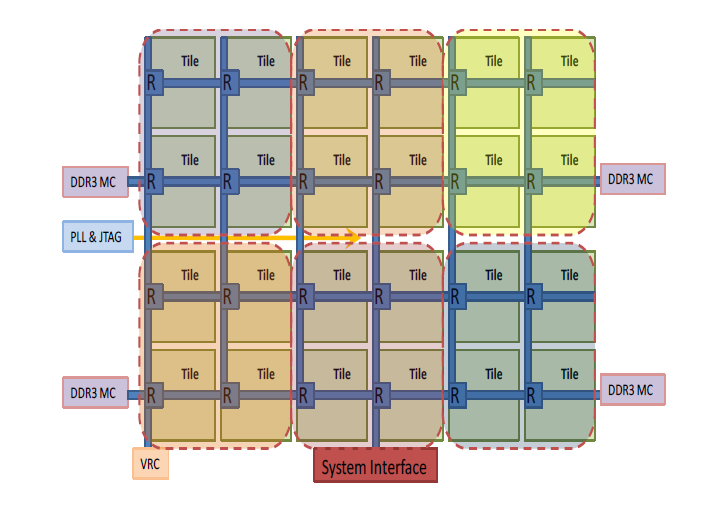
\includegraphics[width=.45\columnwidth]{SCCBlockDiagram.png}
    \end{figure}
  
\end{frame}


\begin{frame}
	\frametitle{Piattaforma di sviluppo}

	Oltre all'SCC, comprende
	\begin{itemize}
		\item un FPGA che fa da chipset per l'SCC
		\item un \emph{Board Management Controller} per il controllo delle funzionalit� critiche della piattaforma
		\item una workstation operativa (MCPC)
	\end{itemize}

	\begin{figure}
      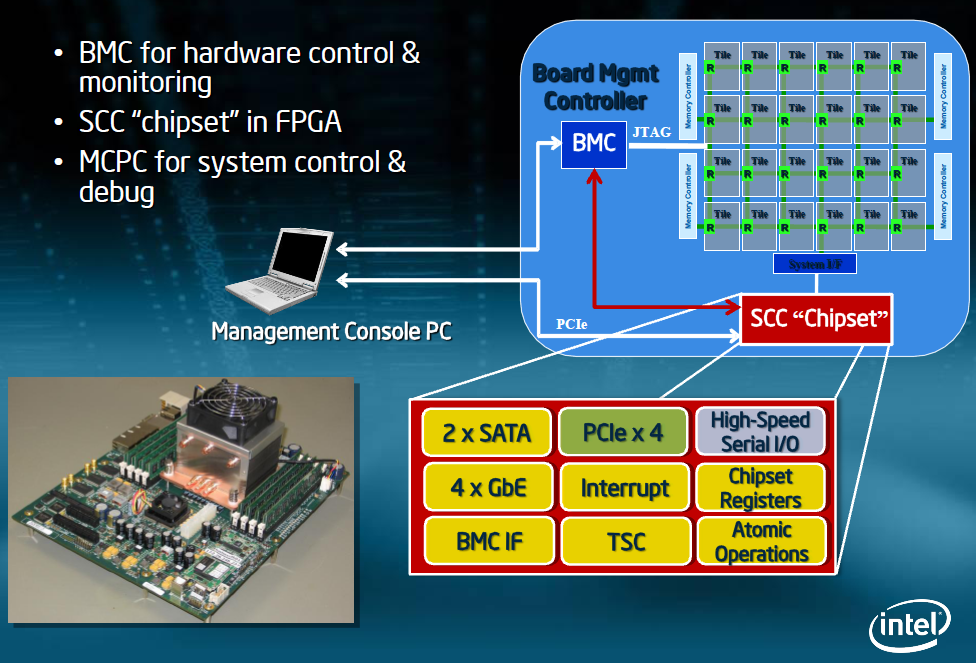
\includegraphics[width=.45\columnwidth]{RockyLake.png}
    \end{figure}
\end{frame}  


\begin{frame}

  \frametitle{Architettura del tile}

		\begin{enumerate}
			\item due IA core PC54C, con cache L1 interna e cache L2 esterna
			\item un crossbar router a 5 porte, che interfaccia il tile con la mesh 
			\item una \emph{mesh interface unit} (MIU) che gestisce tutti gli accessi alla memoria e le operazioni di scambio dei messaggi
			\item una \emph{memory lookup table} (LUT) che permette la traduzione degli indirizzi fisici del core in indirizzi di sistema (globali)
			\item un message-passing buffer, che supporta lo scambio di messaggi.
			\item ciruciterie di generazione e raccordo del clock (GCU e CCF)
	\end{enumerate}

\end{frame}

\begin{frame}
	\frametitle{Architettura del tile}

	\begin{figure}
      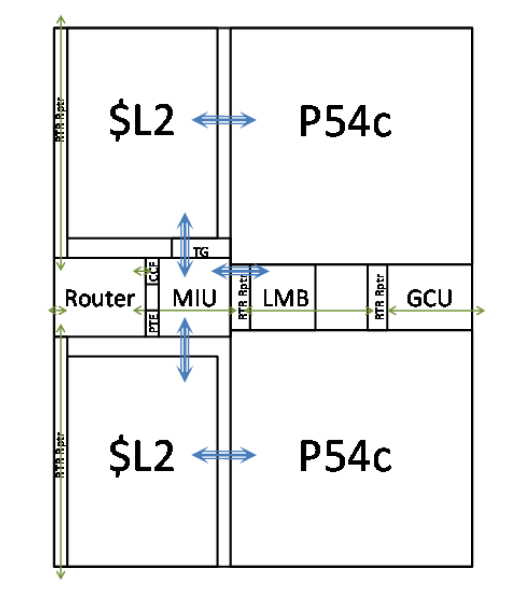
\includegraphics[width=.45\columnwidth]{Tile.png}
    \end{figure}
\end{frame}  


\begin{frame}

  \frametitle{Supporto allo scambio di messaggi}
	
	\begin{block}{Message passing buffer}
		16 KB di SRAM accedibile da qualsiasi core, da utilizzarsi preferibilmente come memoria tampone durante lo scambio di messaggi
	\end{block}

	\begin{block}{Modifiche principali al core P54C}
		\begin{itemize}
			\item aggiunta di un nuovo tipo di memoria, MPBT (message passing buffer type)
			\item aggiunta dell'istruzione CL1INVMB per invalidare le linee di L1 cache di tipo MPBT
			\item aggiunta di un write combine buffer verso il bus di memoria, che agisce sui dati di tipo MPBT
		\end{itemize}
	\end{block}

\end{frame}


\begin{frame}
	\frametitle{Tabelle di lookup}
	
	Permettono di tradurre gli indirizzi fisici su 32 bit di un core in indirizzi di sistema a 46 bit.
	\begin{figure}
      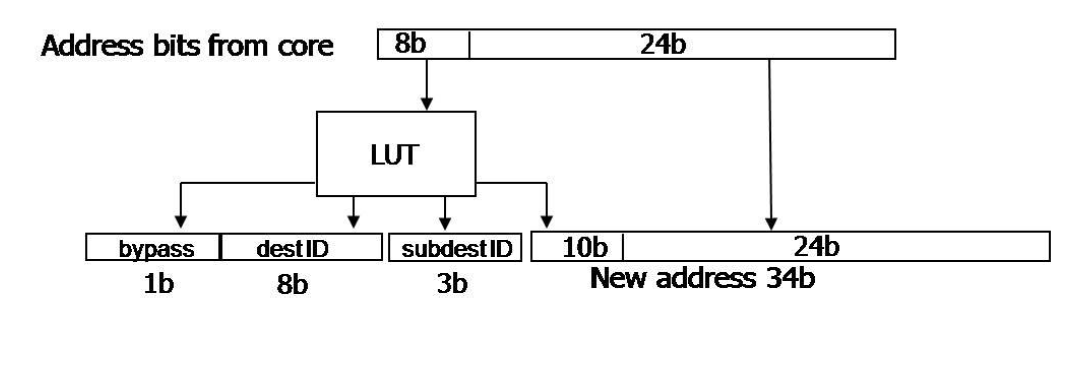
\includegraphics[width=.85\columnwidth]{LUT.png}
    \end{figure}
\end{frame}  


%=================================================================
\section{Programmazione con l'SCC}
%=================================================================

\begin{frame}

  \frametitle{Libreria RCCE}

  \begin{block}{Caratteristiche}
		\begin{itemize}
			\item libreria minimale e di basso livello che permette ai core dell'SCC di comunicare scambiandosi messaggi
			\item concepita inizialmente per lavorare sull'SCC in mancanza di sistema operativo
			\item primitive di invio e ricezione bloccanti
			\item non utilizza il meccanismo delle interruzioni
			\item molto efficiente (niente servizi di sistema, primitive bloccanti)
			\item due interfacce: una di pi� alto livello (\emph{nongory}) e l'altra di pi� basso livello (\emph{gory})
		\end{itemize}
	\end{block}

\end{frame}

\begin{frame}

  \frametitle{Libreria RCCE}

  \begin{block}{ Modello offerto al programmatore (\emph{nongory}) }
		\begin{itemize}
			\item ad ogni core tra gli N coinvolti nell'elaborazione � assegnato un \emph{rank} diverso (intero tra 0 ed N-1)
			\item le primitive \texttt{RCCE\_send()} e \texttt{RCCE\_receive()} permettono di inviare/ricevere un numero di byte arbitrario verso/da un altro core
			\item il programmatore deve attenersi al modello SPMD (\emph{Single Program Multiple Data)}
			\item su ciascun core non possono essere lanciate contemporaneamente pi� applicazioni che utilizzano RCCE (o l'MPB)
		\end{itemize}
	\end{block}

\end{frame}



\begin{frame}

  \frametitle{Libreria RCCE}

  \begin{block}{ Implementazione (\emph{nongory}) }
		\begin{itemize}
			\item modello di allocazione simmetrica delle variabili nell'MPB
			\item due array di flag di sincronizzazione per ogni core, l'array \texttt{sent} e l'array \texttt{ready}, aventi ciascuno N elementi
			\item la sincronizzazione avviene in modo semplice con un protocollo basato sulle attese attive
			\item due implementazioni dei flag possibili, con diversi overhead spaziali e temporali
		\end{itemize}
	\end{block}

\end{frame}



%=================================================================
\section{Algoritmo genetico parallelo}
%=================================================================

\begin{frame}
	\frametitle{Algoritmo genetico}

	\only<1>{
		\begin{block}{Definizione}
		\'E un algoritmo stocastico di ottimizzazione \emph{population-based}.
		L'evoluzione avviene per mezzo di
		\begin{enumerate}
			\item selezione
   		\item crossover (ricombinazione)
			\item mutazione
		\end{enumerate}	
		\end{block}
	}

	\only<2>{
		\begin{block}{Altre caratteristiche dell'algoritmo}
		\begin{itemize}
			\item fitness scaling
   		\item elite children
			\item inizializzazione della popolazione iniziale in modo casuale
			\item condizioni di terminazione (numero di iterazioni, varianza della popolazione)
		\end{itemize}	
		\end{block}
	}

\end{frame}



\begin{frame}
	\frametitle{Parallelizzazione dell'algoritmo genetico}
	
	\only<1>{
		\begin{block}{Modelli di parallelizzazione}
		\begin{enumerate}
			\item Master-slave (sincronizzato/asincrono)
			\item Static subpopulation with migration
			\item Overlapping subpopulation without migration
			\item Massively parallel genetic algorithms
		\end{enumerate}	
		\end{block}
	}

	\only<2>{
		\begin{block}{}
			Il modello con sottopopolazioni e migrazioni � quello pi� adatto all'architettura ibrida dell'SCC.
		\end{block}

		\begin{block}{}
			Si alternano fasi di evoluzione isolata (algoritmo sequenziale) a fasi di migrazioni.
		\end{block}
	}

	\only<3>{
		\begin{block}{Estensioni necessarie per la parallelizzazione}
			\begin{itemize}
				\item individuazione di uno schema di migrazione
				\item individuazione di un algoritmo di terminazione distribuita
			\end{itemize}
		\end{block}
	}

\end{frame}


\begin{frame}
	\frametitle{Schema di migrazione}
	
	\only<1>{
		Specifica come il materiale genetico localmente dominante viene scambiato tra i core durante una fase di migrazione.
		\begin{block}{Schema a flusso circolare unidirezionale}
		\begin{itemize}
			\item ciascun core ha un core precedente ed un successivo
			\item durante una fase di migrazione ciascun core riceve dal precedente e invia al successivo
			\item ciascun core ha un colore che determina l'ordine degli scambi
			\item due parametri da specificare: \emph{migration} fraction e \emph{migration period}
			\item migrazione in due o tre passi (primitive bloccanti)
			\item si evitano deadlock
		\end{itemize}	
		\end{block}
	}

	\only<2>{
		\begin{block}{Esempio}
			\begin{figure}
	      	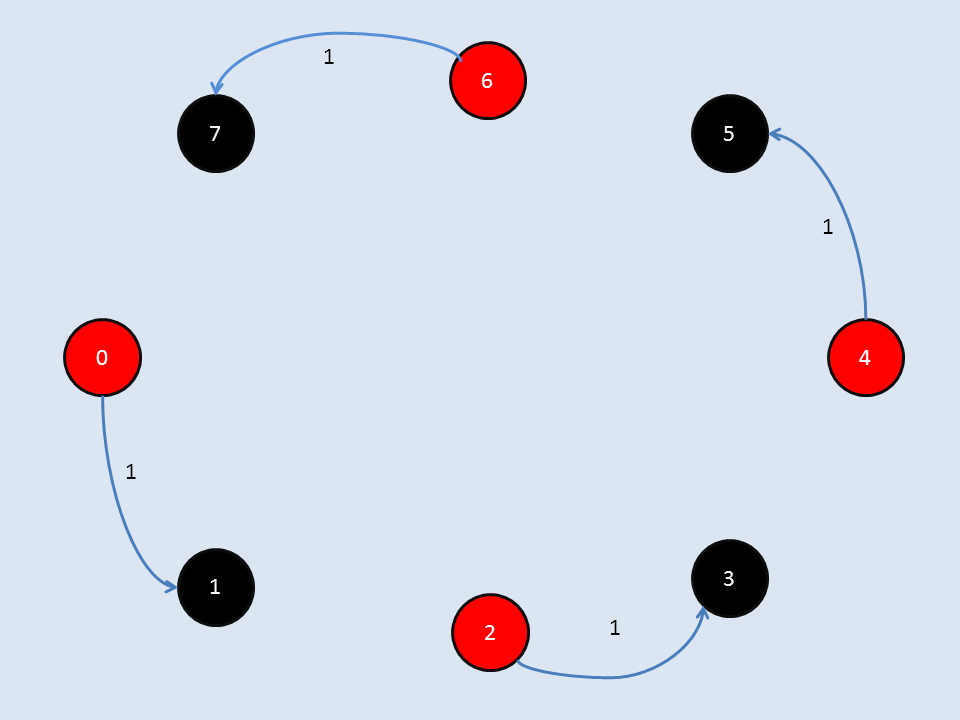
\includegraphics[width=.65\textwidth]{migrPari1.png}
	    	\end{figure}
		\end{block}
	}

	\only<3>{
		\begin{block}{Esempio (continua)}
			\begin{figure}
	      	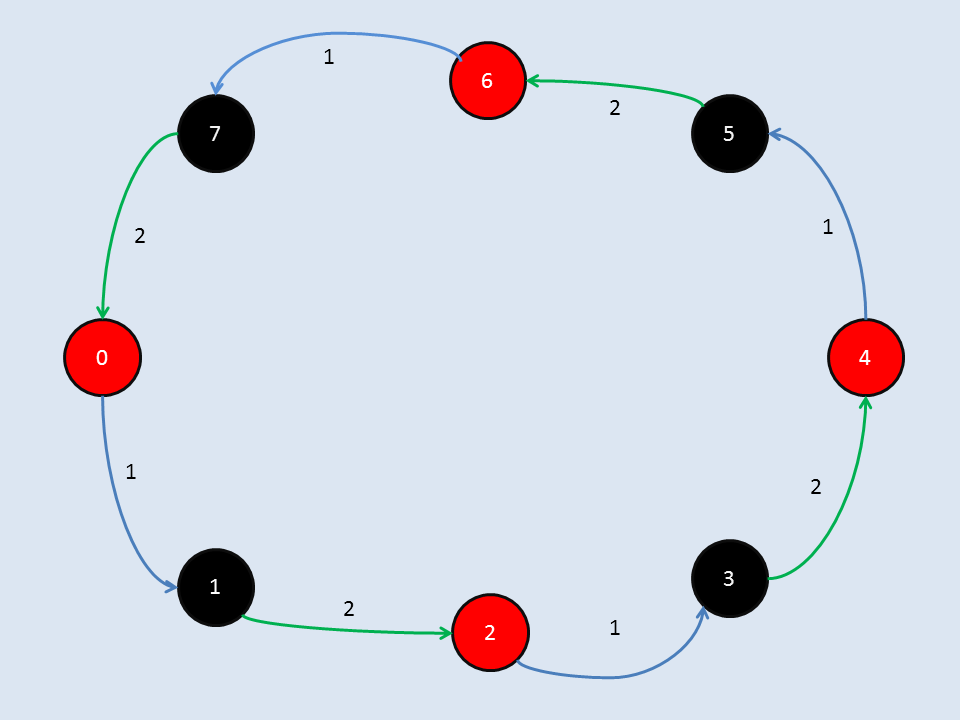
\includegraphics[width=.65\textwidth]{migrPari2.png}
	    	\end{figure}
		\end{block}
	}

	\only<4>{
		\begin{block}{Ricerca di cicli hamiltoniani bilanciati sull'SCC}
		Problema semplice, in quanto il grafo � completamente connesso.
		\end{block}

		\begin{block}{}
		I core disponibili possono essere solamente un sottoinsieme di quelli totali.
		Si cercano cicli il pi� possibile \emph{bilanciati}:
		\begin{enumerate}
			\item scelta di percorsi ottimi in casi particolarmente favorevoli
			\item euristica da applicare nei restanti casi
		\end{enumerate}	
		\end{block}
	}

	\only<5>{
		\begin{block}{Esempio ciclo ottimo}
			\begin{figure}
	      	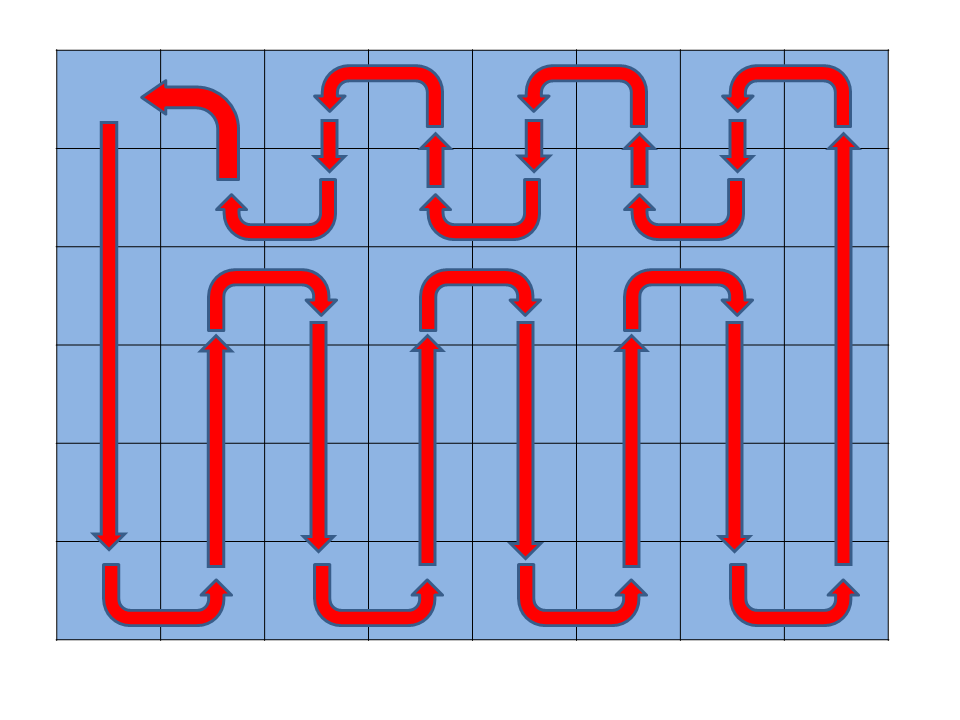
\includegraphics[width=.65\textwidth]{verticalTilesPath.png}
	    	\end{figure}
		\end{block}
	}

	\only<6>{
		\begin{block}{Euristica da applicare nel caso generale}
			\begin{figure}
	      	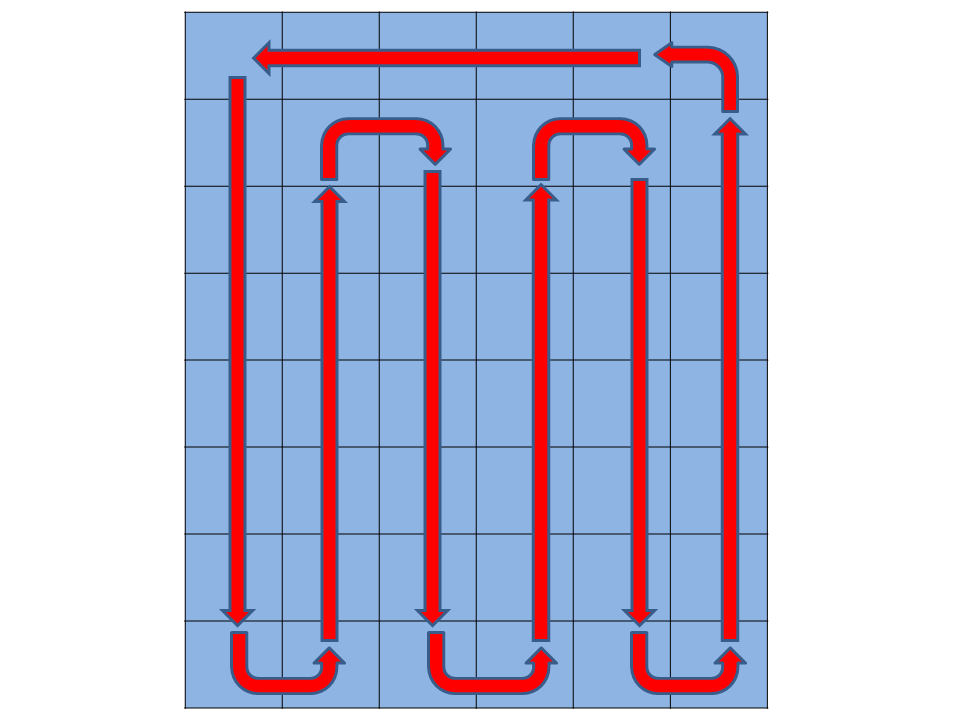
\includegraphics[width=.65\textwidth]{genPath.png}
	    	\end{figure}
		\end{block}
	}

\end{frame}

\begin{frame}

	\frametitle{Algoritmo distribuito di terminazione}
	
	\only<1>{
		\begin{block}{Problemi}
			\begin{itemize}
				\item i core possono convergere in iterazioni diverse
				\item una fase di migrazione non pu� essere eseguita solo da un sottoinsieme di core
				\item si pu� terminare solo quando tutti i core sono arrivati a convergenza
				\item si vuole evitare di appesantire le comunicazioni
			\end{itemize}	
		\end{block}
	}

	\only<2>{
		\begin{block}{Soluzione}
			\begin{itemize}
				\item protocollo di segnalazione che agisce solo durante le fasi di migrazione
				\item ogni nodo segnala la propria decisione di terminare al nodo successivo
				\item tutti i core terminano esattamente durante la prima fase di migrazione in cui la terminazione � possibile
				\item necessit� di un nodo coordinatore
				\item implementazione tramite macchina a stati finiti
			\end{itemize}
		\end{block}
	}

	\only<3>{
		\begin{block}{Macchina a stati per il nodo coordinatore}
			\begin{figure}
	      	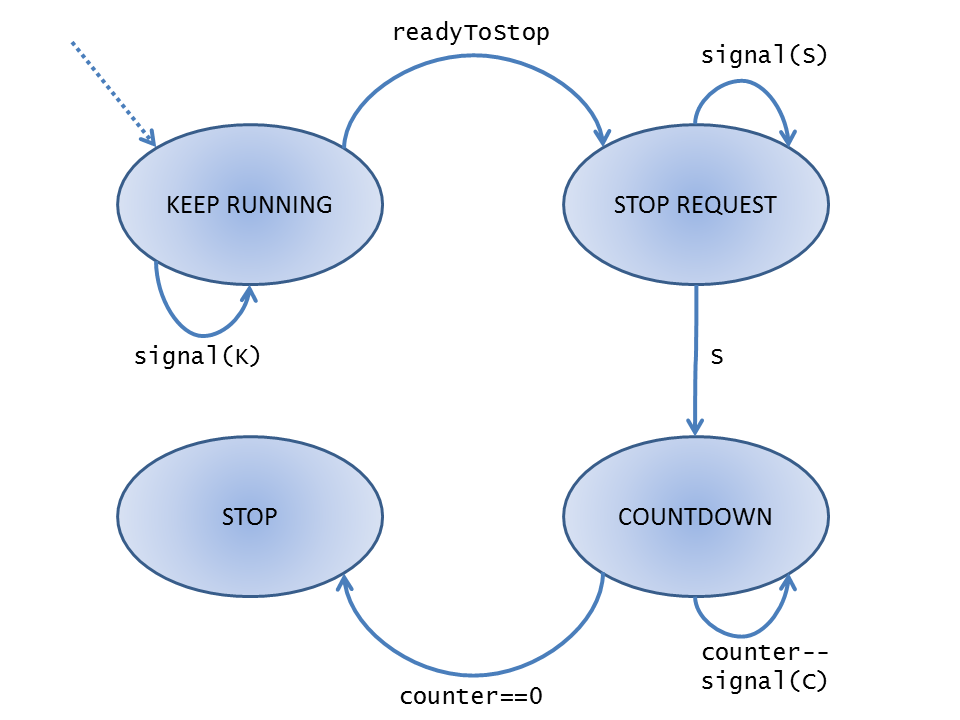
\includegraphics[width=.65\textwidth]{machineCoord.png}
	    	\end{figure}
		\end{block}
	}

	\only<4>{
		\begin{block}{Macchina a stati per un nodo non coordinatore}
			\begin{figure}
	      	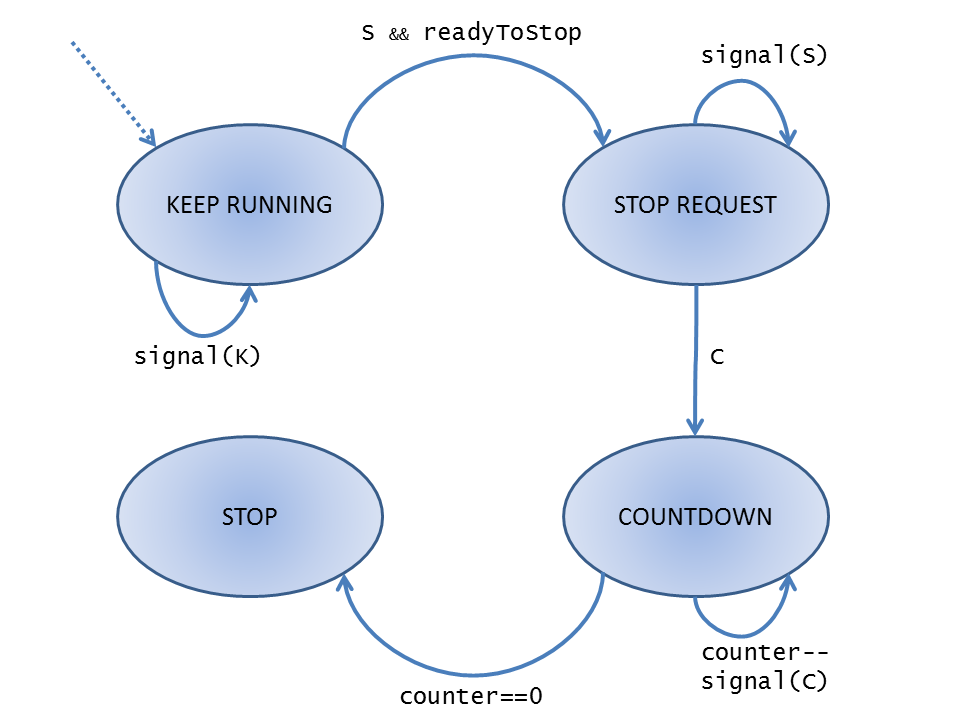
\includegraphics[width=.65\textwidth]{machineNormal.png}
	    	\end{figure}
		\end{block}
	}

\end{frame}





%=================================================================
\section{Risultati delle simulazioni}
%=================================================================

\begin{frame}
	\frametitle{Addestramento di una rete neurale}

	\only<1>{
		\begin{block}{Problema test}
			Addestramento di una rete neurale feed-forward
			\begin{itemize}
				\item dataset con ingresso ed uscita unidimensionale, composto da 50 elementi
				\item minimizzazione della deviazione standard dell'errore sul dataset
				\item 4 neuroni nascosti con funzione di attivazione sigmoidale
				\item neurone nello strato di uscita con funzione di attivazione lineare
				\item il test ha solo scopo dimostrativo, e pertanto non sono state applicate tecniche di cross-validation
				\item il dominio di ricerca � $\R^{13}$
			\end{itemize}
		\end{block}
	}

	\only<2>{
		\begin{block}{Parametri dell'algoritmo genetico}
			\begin{itemize}
				\item massimo numero di iterazioni: 5000
				\item crossover fraction: 0.8
				\item numero di elite children: 3
				\item migration fraction: 0.1
				\item migration period: 20 iterazioni
				\item shrink factor: 1.0
			\end{itemize}
		\end{block}
	}

	\only<3>{
		\begin{block}{Dataset 1}
			\begin{figure}
	      	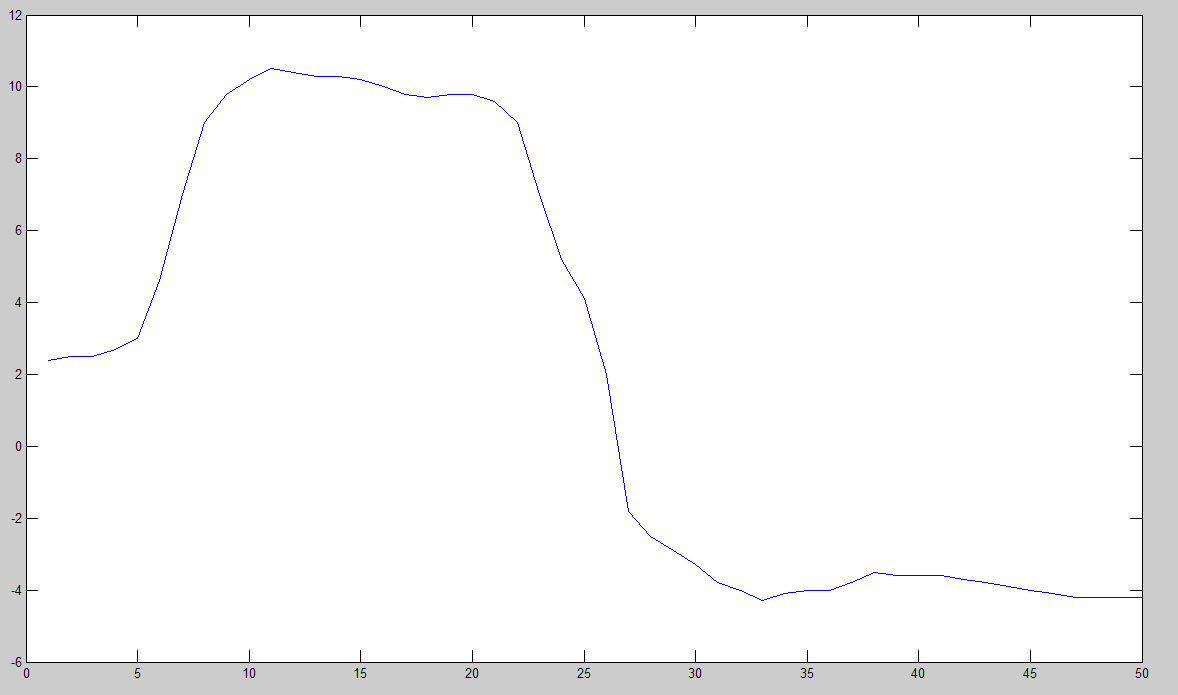
\includegraphics[width=.65\textwidth]{dataset1.png}
	    	\end{figure}
		\end{block}
	}

	\only<4>{
		\begin{block}{Risultati sul dataset 1} 
			\begin{itemize}
				\item intervallo di inizializzazione: [-10,10]
				\item dimensione della popolazione: 20
			\end{itemize}
			\begin{figure}
	      	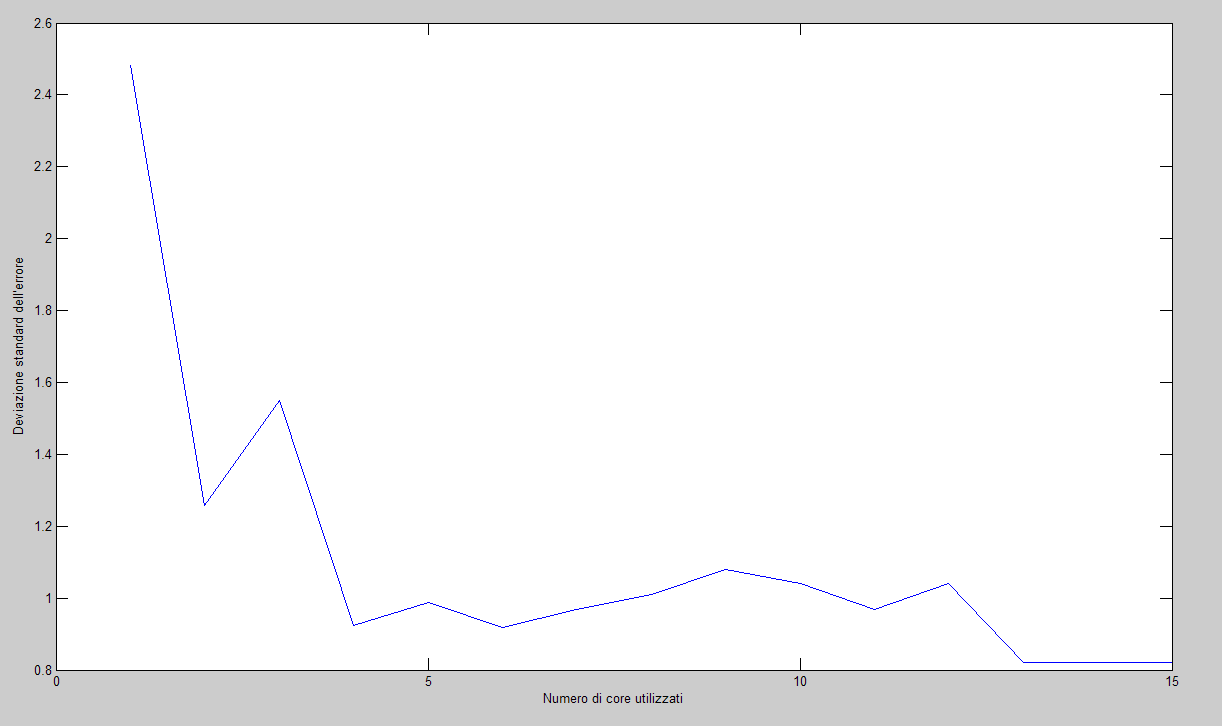
\includegraphics[width=.55\textwidth]{grafico1.png}
	    	\end{figure}
		\end{block}
	}

	\only<5>{
		\begin{block}{Dataset 2}
			\begin{figure}
	      	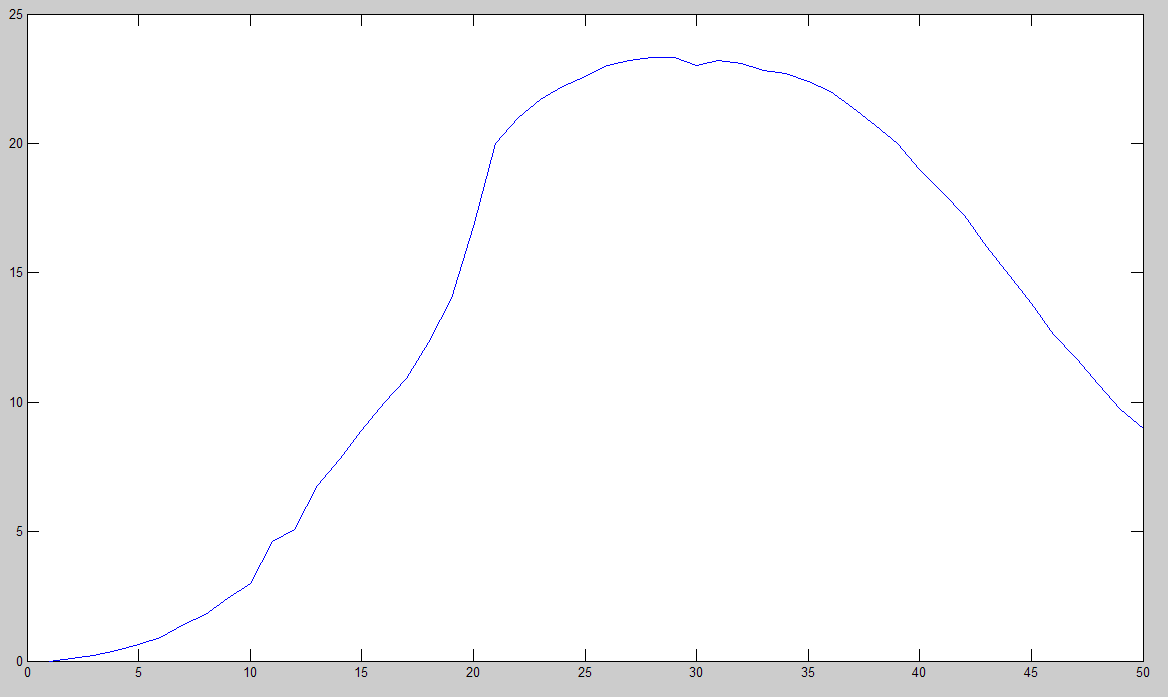
\includegraphics[width=.65\textwidth]{dataset2.png}
	    	\end{figure}
		\end{block}
	}

	\only<6>{
		\begin{block}{Risultati sul dataset 2}
			\begin{itemize}
				\item intervallo di inizializzazione: [-30,30]
				\item dimensione della popolazione: 80
			\end{itemize}
			\begin{figure}
	      	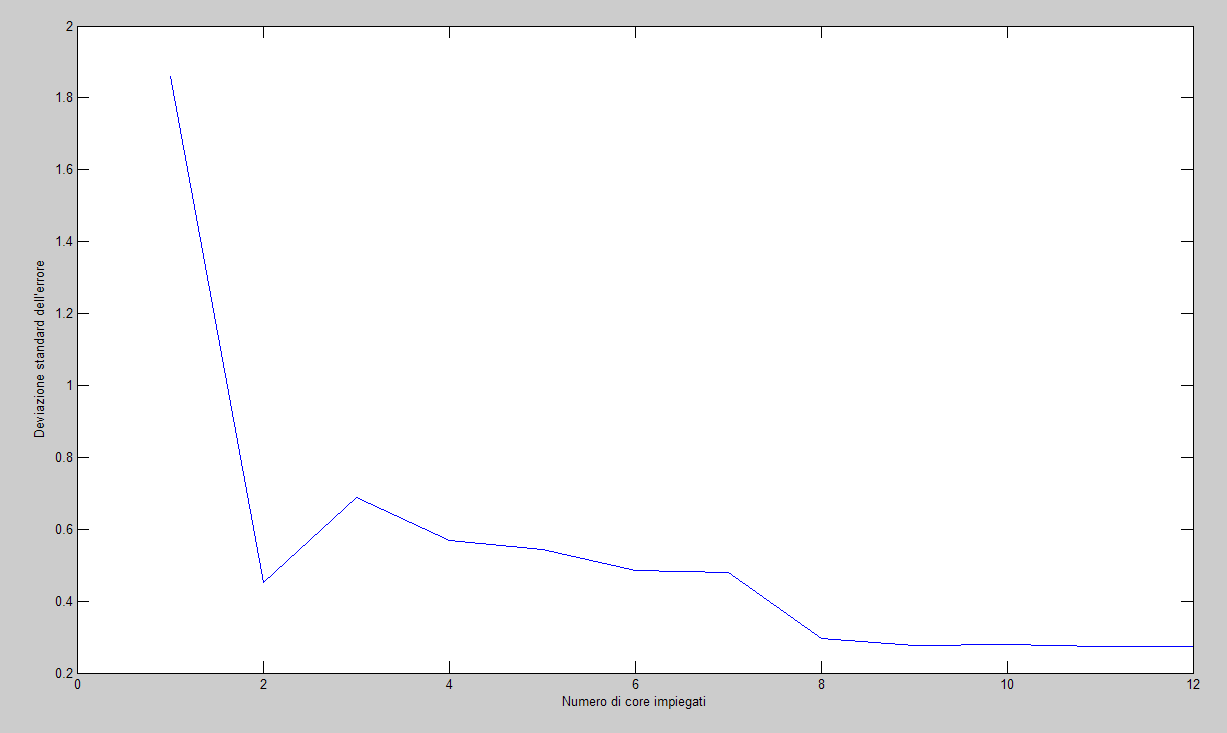
\includegraphics[width=.55\textwidth]{grafico2.png}
	    	\end{figure}
		\end{block}
	}

	\only<7>{
		\begin{block}{Considerazioni sui risultati}
			\begin{itemize}
				\item tempo di esecuzione indipendente dal numero di core impiegati
				\item l'intervallo di inizializzazione va dimensionato in base al numero di core e alla dimensione della popolazione
				\item la probabilit� di convergere a buone soluzioni diminuisce se si ingrandiscono gli intervalli iniziali
				\item la stessa probabilit� aumenta se si aumenta il numero di core e/o la dimensione della popolazione
				\item intervalli troppo piccoli rendono inutile l'utilizzo di tanti core
				\item necessit� di trovare un buon compromesso
			\end{itemize}
		\end{block}
	}	

\end{frame}


\end{document}
